% !TEX root = rapport.tex
\section{Current}
\label{current}
% Kolla upp hur utgågna patent på current devices spelar in, det verkar vara en faktor på åtminstånde touch screen, kan säkert vara intressant på voice också.
% Brasklapp om att våra slutsatser bara gäller det vi har hittat och att vi inte garanterar att all relevant information är med
% Fundamentals: Asmycket referenser i kapitel 1.4
\todo{kommentarer om utgångna patent och referenser i fundamentals.}

Several input devices in this paper such as the keyboard and the mouse, are still wildely used but can be seen as historical devices. This is justified by the fact that they remain largely unchanged - if not in their physical design then in the fashion they are used [citation needed] \todo{ref}. On the other hand, a number of other input/output devices that can be seen as to be recent have a long history behind them. taken a larger and larger market share. Although \emph{touchpads}, \emph{touchscreens} and \emph{speech recognition} techniques were researched as far back as the 1960's \cite{buxton}\cite{shoebox}, they have only now began to see commercial use and have likely still not reached their "peak". 


\subsection{Touch devices}
Touchscreen devices have become increasingly popular during the last years, through the breakthrough of \emph{smart devices} (i.e. smart phones and tablets) running specialized operating systems such as the Apple's iOS and Google's Android. The technology used in these devices however, have evolved over over a much longer time.

One of the first mentions of touchscreens was by E.A. Johnson in 1965, describing a touchscreen and identifying some potential uses in a short article, less than a single page\cite{4205802}. Some of the earliest developed systems came in the beginning of the 1970's. Early prototypes are the PLATO IV\cite{buxton} (1972) (seen in figure \ref{platoIV}) and a transparant touchscreen was developed and put to use by CERN in 1973\cite{cern}.

% http://cooper.library.uiuc.edu/archives/archon/?p=digitallibrary/digitalcontent&id=1478
% NOTE: USE OF THIS PICTURE HAS NOT BEEN APPROVED. I'VE EMAILED THE UNIVERSITY
% OF ILLINOIS, AND I'M AWAITING REPLY.
\begin{figure}[]
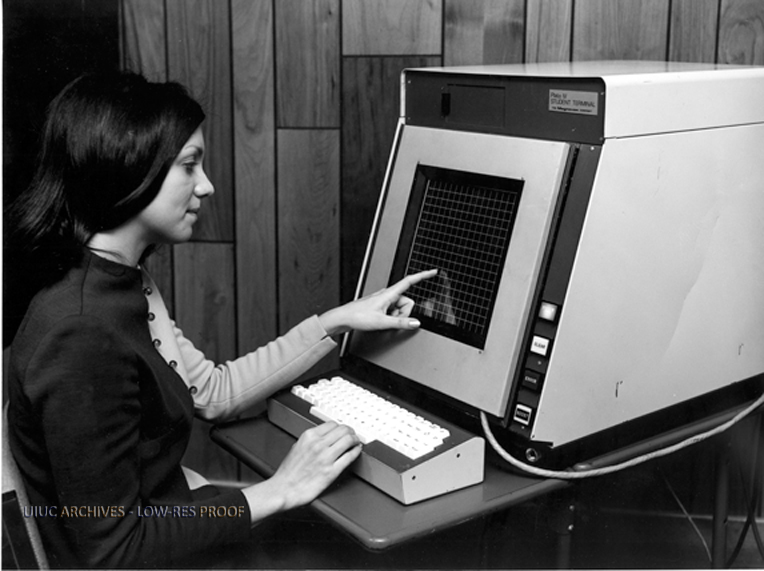
\includegraphics[width=0.8\textwidth] {bilder/platoiv.jpg}
\caption{Student using the PLATO IV.}
\label{platoIV}
\end{figure}
% Bild på plato
\nocite{platoiv}
\todo{enligt kommentaren är denna bild inte approved.}

%These devices used METOD - PROBLEM MED DETTA - BESKRIVA NÄSTA GENERATION. (DET SKA HANDLA OM LJUS HÄR, JAG REFERERAR TILL DETTA OSKRIVNA STYCKE SENARE.
\todo{kommentar om ljus och ett oskrivet stycke.}

The initial uses of touchscreens were point-to-select systems used in for example ATM machines or cash registers in restaurants and were relatively non-demanding on the screen performance\cite{buxton}. But there were also early attemps to make \emph{PDAs}\footnote{Personal Digital Assistant}. The first products to enter the market were the Palm Zoomer and the IBM Simon. The Simon was a mobile phone without any physical buttons, having only a touchscreen as its working area. But beyond regular telephone capabilities, it could also manage information such as a telephone book and be used for drawing and taking notes. Due to this, it is sometimes refered to as the first \emph{smartphone}\cite{buxton}.

Smartphones have seen much development since the release of Simon, and today (2013) it is estimated that more than a billion people use smartphones\cite{billion1}\cite{billion2}. This is largely due to the recent popularisation of the apple iOS and the android operating system[Reference needed]. 

This increase in the number of touch-based devices has changed the way in which we interact with computers. New operating systems especially designed for smartphones and other smart devices, such as the popular IOs and Android operating systems have a fundamentally different approach to computer interaction.

The traditional WIMP approach requires the user to find the cursor on the display, move it to the desired location and click the mouse button to interact, or use the keyboard to input data. The touch screen on the other hand gives the user the ability to point directly at the desired item at the screen to activate it. An on-screen keyboard appears only when it is needed, allowed the computers to show only what is relevant at any point of time. This has made computers so portable that they can be used in almost any context and in a user friendly way [JAG TROR JAG KAN HITTA EN BRA REFERENS I MIN HCI-BOK]\todo{referens}. The tablet is so simple in its design that it can be used by small kids and even cats [Bild på frasse tagen med en smartphone. Prata om att smart devices gör saker som att ta bilder]\todo{frasse och ta bilder}.

One of the big breakthroughs that has allowed the touch screen to become the only input device required by a computer is the introduction of multi finger gestures. While touch screens previously only handled one action ("left mouse button"), the use of multi hand gestures removes the need for icons. The rest of the functionality can be reached by for example pinching or swiping one's fingers. This type of interaction is not fundamentally more user-friendly, but it can be if used in the right way.

\begin{figure}[]
\includegraphics[width=0.8\textwidth] {bilder/ipadbook.jpg}
\caption{Apple Ipad showing iBooks, with the book Alice's Adventures in Wonderland.}
\label{ibooks}
\end{figure}
% Bild på xerox-musen eller mac-musen
\nocite{ipadbook}

Consider a common application of a smart device, that of reading an e-book on a tablet. On a traditional computer, one typically reads the e-book as a document, with all pages following each other from top to bottom. On the tablet, the e-book can be made to look like a book, see figure \ref{ibooks}. The act of swiping one's finger from right to left triggers the book to turn the page, similar to what one would do in a physical book. This could be done with another gesture, for example by drawing a circle on the screen or triple-tapping an so on, but these approaches would not at all be as intuitive as the swipe-gesture.

\todo{skriv något om gyrosensorer (Å: tre dimensioner) och dylikt som används av smart devices}

\subsection{Voice recognition}

Voice recognition is another input method that has become increasingly popular during the last years. This input method uses speech recognition by analyzing input from a microphone. One the spoke word has been analysed, it can be used in several ways.

One ambition is that of providing real-time subtitles to spoken text, for example to aid those with hearing disorders. As an input method, the sound input can be parsed by the computer and then trigger a predefined action. This type of speech recognition has recently seen big progress, although it has not yet seen widespread use. For example, in the past year (2012) Microsoft presented an English to synthesised speech Chinese translator, working in real time.

\subsection{Typ en egen subsection}\todo{ge mig ett namn}

While the computers have become powerful and cheap enough to make speech recognition broadly available recently, its history is much longer. The first working implementation was introduced by Bell Labs in 1952. The system was able to recognise spoken language at telephone quality, and had a success rate of between 97-99 \cite{Davis52}.

Early speech recognition attemps were simple, and could not analyse sentences. Instead, single words were compared to a rather small dictionary, compared to those used today. The Bell Labs system from 1952 was able to recognise the numbers 0 to 9, spoken by a single speaker.[citation B.H. Juang - Automatic Speech Recognition – A Brief History of the Technology Development]\todo{referens} The user was forced to make a small pause between every word for the system to recognize them. 

Another system worked by analysing phonems in the spoken text. Phonemes are the smallest building blocks of the language and consist of the individual sounds used to construct words and sentences[REFERENS TILL KOG.PSYK-boken]\todo{referens}. Early phonem-based techniques could only recognise a subset of phonemes. RCA Labs in 1956 could recognise 10 phonemes, spoken by a single speaker. Fry and Denes at the University College in England could recognise 4 wovels and 9 consonants. More notably, they were the first to incorporate statistical information in the analysis[Juang]\todo{referens} - something that now is fundamental in speech recognition. By analyzing speech at this low level the system becomes less dependant on pauses and dialect in speech.

In the 1980's, the use of \emph{Hidden Markov Models} was introduced in speech recognition\cite{rabiner1986introduction}. Hidden Markov models are statistical Markov models where the path through the process is not observable. The Markov Models use previously gathered statistical data to with some certainty guess which phoneme the user is saying, and the chain of phonemes considered to be correct are then matched to a phoneme-word database to decide which word the user has spoken. The context of the word is also taken into acount to prevent homonyms of the desired word to be entered instead. The Markov Model Speech Recognition systems "learn" the users voice and speech patterns by using the data from corrections to alter the statistics used to decide which phoneme was spoken. 

This next part will explain what markow chain thingies are, with a reference to the picture.\todo{unwritten part about markow chains}

\begin{figure}[]
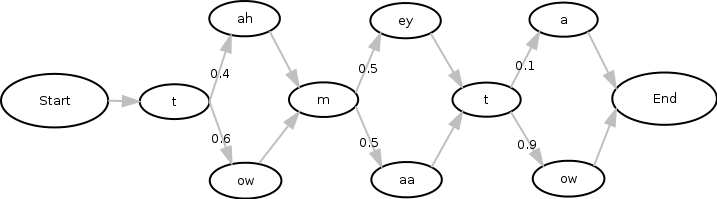
\includegraphics[width=0.8\textwidth] {bilder/tomato.jpg}
\caption{A model describing the statistical values of phoneme input of the word \emph{tomato}. The model contains american and british english pronounciations, with a small statistical favor of the british accent.}
\label{ibooks}
\end{figure}

Most speech recognition software today use Hidden Markov Chains for speech analysis\cite{DNN}, but recent research has shifted focus towards the user of a type of artificial neural network, called Deep Neural Networks (DNN). Neural networks have been used for speech recognition since the late 80's, but the use of DNN is the first that has been shown to have substantial benefits over the use of the traditional markov chain approach. A research collaboration around DNN exists between the University of Toronto, Microsoft, IBM and Google. Late 2012, Microsoft publicly demonstrated their work with speech recognition - a system that can translate spoken English into spoken Mandarin in real time and in the voice of the speaker. In conjunction with the demonstration, Microsofts chief researcher Rick Rashid says about DNNs: "While still far from perfect, this is the most dramatic change in accuracy since the introduction of hidden Markov modeling in 1979"\cite{chin}.

In the 1990:s personal computers became fast enough to power speech recognition software.
\todo{oavslutat stycke}

Referens BLABLA:
A. Waibel, T. Hanazawa, G. Hinton, K. Shikano, and K. J. Lang, (1989) "Phoneme recognition using time-delay neural networks," IEEE Transactions on Acoustics, Speech and Signal Processing, vol. 37, pp. 328-339. \todo{vilsekommen referens}
